\documentclass[1p]{elsarticle_modified}
%\bibliographystyle{elsarticle-num}

%\usepackage[colorlinks]{hyperref}
%\usepackage{abbrmath_seonhwa} %\Abb, \Ascr, \Acal ,\Abf, \Afrak
\usepackage{amsfonts}
\usepackage{amssymb}
\usepackage{amsmath}
\usepackage{amsthm}
\usepackage{scalefnt}
\usepackage{amsbsy}
\usepackage{kotex}
\usepackage{caption}
\usepackage{subfig}
\usepackage{color}
\usepackage{graphicx}
\usepackage{xcolor} %% white, black, red, green, blue, cyan, magenta, yellow
\usepackage{float}
\usepackage{setspace}
\usepackage{hyperref}

\usepackage{tikz}
\usetikzlibrary{arrows}

\usepackage{multirow}
\usepackage{array} % fixed length table
\usepackage{hhline}

%%%%%%%%%%%%%%%%%%%%%
\makeatletter
\renewcommand*\env@matrix[1][\arraystretch]{%
	\edef\arraystretch{#1}%
	\hskip -\arraycolsep
	\let\@ifnextchar\new@ifnextchar
	\array{*\c@MaxMatrixCols c}}
\makeatother %https://tex.stackexchange.com/questions/14071/how-can-i-increase-the-line-spacing-in-a-matrix
%%%%%%%%%%%%%%%

\usepackage[normalem]{ulem}

\newcommand{\msout}[1]{\ifmmode\text{\sout{\ensuremath{#1}}}\else\sout{#1}\fi}
%SOURCE: \msout is \stkout macro in https://tex.stackexchange.com/questions/20609/strikeout-in-math-mode

\newcommand{\cancel}[1]{
	\ifmmode
	{\color{red}\msout{#1}}
	\else
	{\color{red}\sout{#1}}
	\fi
}

\newcommand{\add}[1]{
	{\color{blue}\uwave{#1}}
}

\newcommand{\replace}[2]{
	\ifmmode
	{\color{red}\msout{#1}}{\color{blue}\uwave{#2}}
	\else
	{\color{red}\sout{#1}}{\color{blue}\uwave{#2}}
	\fi
}

\newcommand{\Sol}{\mathcal{S}} %segment
\newcommand{\D}{D} %diagram
\newcommand{\A}{\mathcal{A}} %arc


%%%%%%%%%%%%%%%%%%%%%%%%%%%%%5 test

\def\sl{\operatorname{\textup{SL}}(2,\Cbb)}
\def\psl{\operatorname{\textup{PSL}}(2,\Cbb)}
\def\quan{\mkern 1mu \triangleright \mkern 1mu}

\theoremstyle{definition}
\newtheorem{thm}{Theorem}[section]
\newtheorem{prop}[thm]{Proposition}
\newtheorem{lem}[thm]{Lemma}
\newtheorem{ques}[thm]{Question}
\newtheorem{cor}[thm]{Corollary}
\newtheorem{defn}[thm]{Definition}
\newtheorem{exam}[thm]{Example}
\newtheorem{rmk}[thm]{Remark}
\newtheorem{alg}[thm]{Algorithm}

\newcommand{\I}{\sqrt{-1}}
\begin{document}

%\begin{frontmatter}
%
%\title{Boundary parabolic representations of knots up to 8 crossings}
%
%%% Group authors per affiliation:
%\author{Yunhi Cho} 
%\address{Department of Mathematics, University of Seoul, Seoul, Korea}
%\ead{yhcho@uos.ac.kr}
%
%
%\author{Seonhwa Kim} %\fnref{s_kim}}
%\address{Center for Geometry and Physics, Institute for Basic Science, Pohang, 37673, Korea}
%\ead{ryeona17@ibs.re.kr}
%
%\author{Hyuk Kim}
%\address{Department of Mathematical Sciences, Seoul National University, Seoul 08826, Korea}
%\ead{hyukkim@snu.ac.kr}
%
%\author{Seokbeom Yoon}
%\address{Department of Mathematical Sciences, Seoul National University, Seoul, 08826,  Korea}
%\ead{sbyoon15@snu.ac.kr}
%
%\begin{abstract}
%We find all boundary parabolic representation of knots up to 8 crossings.
%
%\end{abstract}
%\begin{keyword}
%    \MSC[2010] 57M25 
%\end{keyword}
%
%\end{frontmatter}

%\linenumbers
%\tableofcontents
%
\newcommand\colored[1]{\textcolor{white}{\rule[-0.35ex]{0.8em}{1.4ex}}\kern-0.8em\color{red} #1}%
%\newcommand\colored[1]{\textcolor{white}{ #1}\kern-2.17ex	\textcolor{white}{ #1}\kern-1.81ex	\textcolor{white}{ #1}\kern-2.15ex\color{red}#1	}

{\Large $\underline{11n_{140}~(K11n_{140})}$}

\setlength{\tabcolsep}{10pt}
\renewcommand{\arraystretch}{1.6}
\vspace{1cm}\begin{tabular}{m{100pt}>{\centering\arraybackslash}m{274pt}}
\multirow{5}{120pt}{
	\centering
	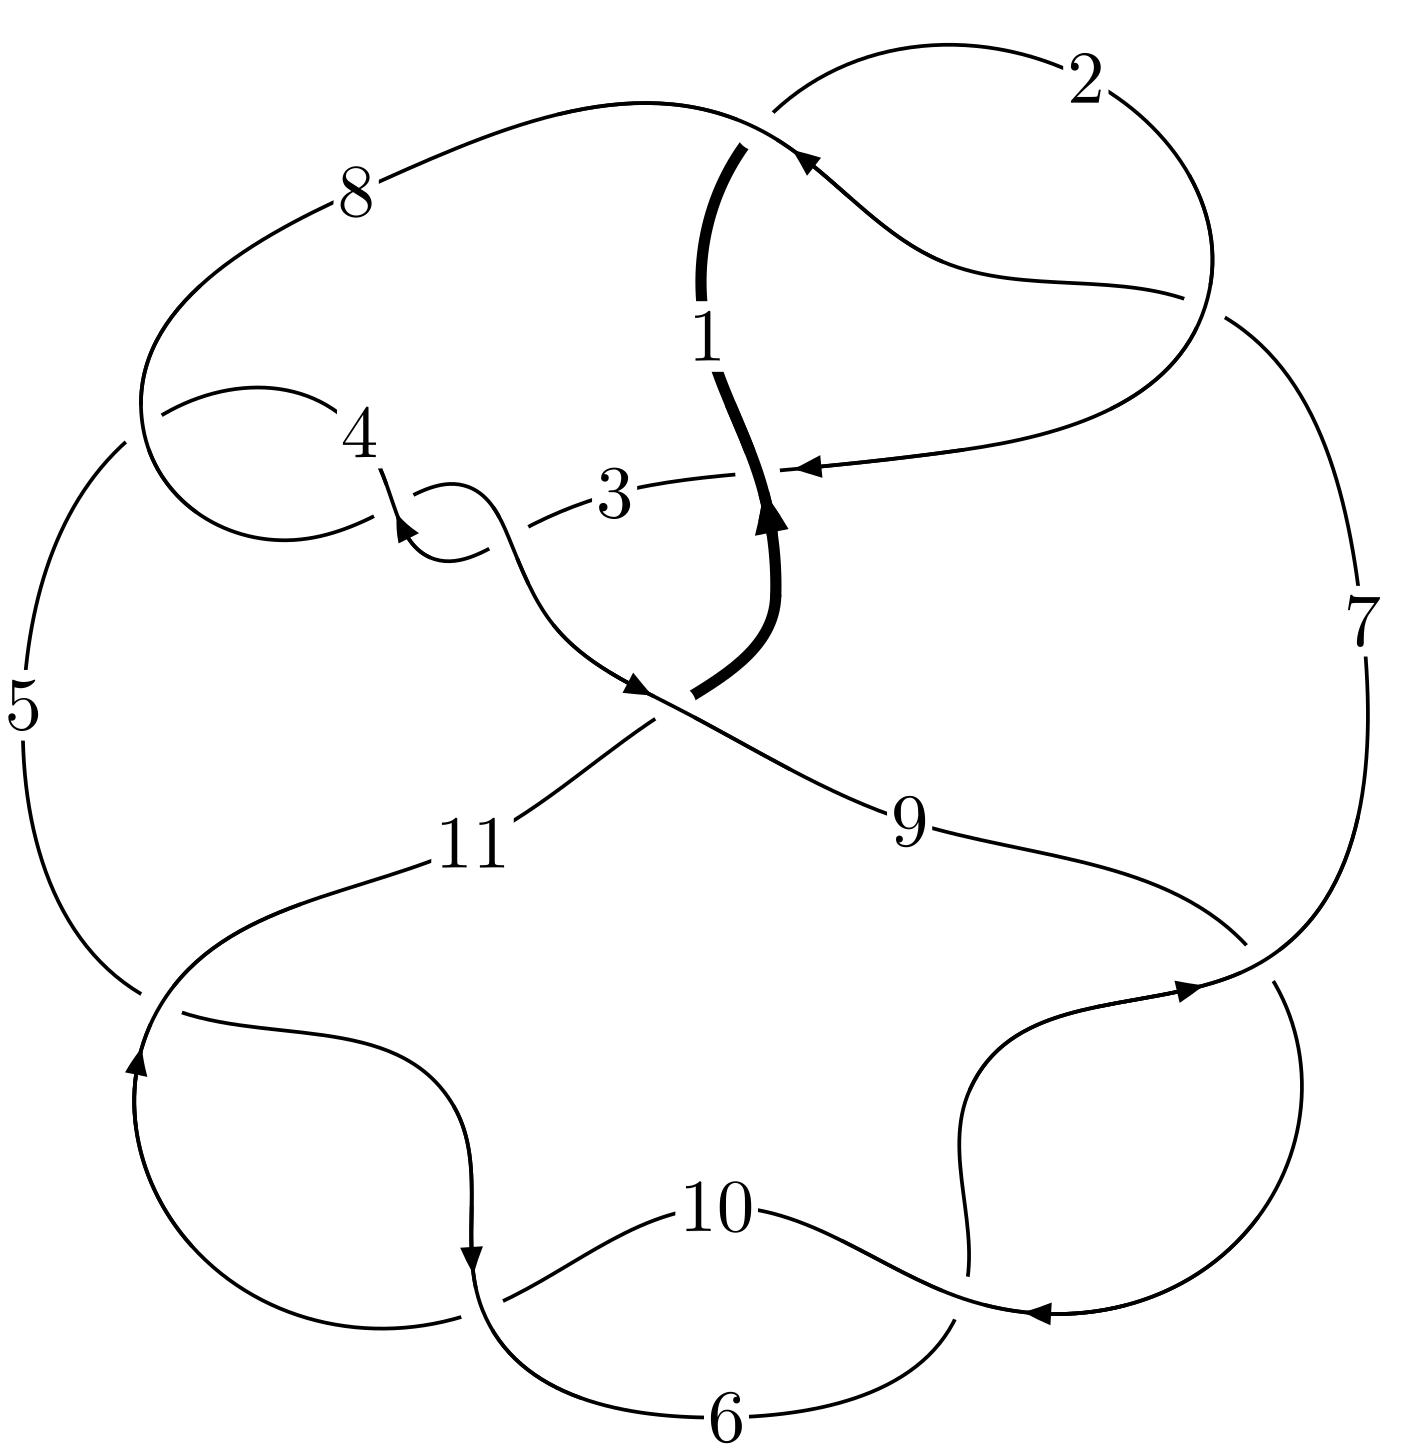
\includegraphics[width=112pt]{../../../GIT/diagram.site/Diagrams/png/756_11n_140.png}\\
\ \ \ A knot diagram\footnotemark}&
\allowdisplaybreaks
\textbf{Linearized knot diagam} \\
\cline{2-2}
 &
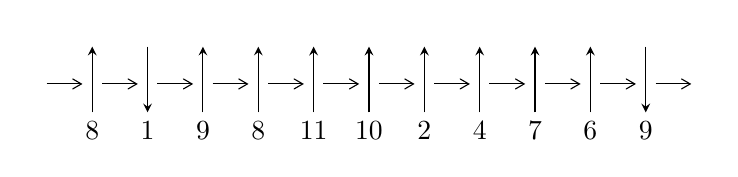
\begin{tikzpicture}[x=20pt, y=17pt]
	% nodes
	\node (C0) at (0, 0) {};
	\node (C1) at (1, 0) {};
	\node (C1U) at (1, +1) {};
	\node (C1D) at (1, -1) {8};

	\node (C2) at (2, 0) {};
	\node (C2U) at (2, +1) {};
	\node (C2D) at (2, -1) {1};

	\node (C3) at (3, 0) {};
	\node (C3U) at (3, +1) {};
	\node (C3D) at (3, -1) {9};

	\node (C4) at (4, 0) {};
	\node (C4U) at (4, +1) {};
	\node (C4D) at (4, -1) {8};

	\node (C5) at (5, 0) {};
	\node (C5U) at (5, +1) {};
	\node (C5D) at (5, -1) {11};

	\node (C6) at (6, 0) {};
	\node (C6U) at (6, +1) {};
	\node (C6D) at (6, -1) {10};

	\node (C7) at (7, 0) {};
	\node (C7U) at (7, +1) {};
	\node (C7D) at (7, -1) {2};

	\node (C8) at (8, 0) {};
	\node (C8U) at (8, +1) {};
	\node (C8D) at (8, -1) {4};

	\node (C9) at (9, 0) {};
	\node (C9U) at (9, +1) {};
	\node (C9D) at (9, -1) {7};

	\node (C10) at (10, 0) {};
	\node (C10U) at (10, +1) {};
	\node (C10D) at (10, -1) {6};

	\node (C11) at (11, 0) {};
	\node (C11U) at (11, +1) {};
	\node (C11D) at (11, -1) {9};
	\node (C12) at (12, 0) {};

	% arrows
	\draw[->,>={angle 60}]
	(C0) edge (C1) (C1) edge (C2) (C2) edge (C3) (C3) edge (C4) (C4) edge (C5) (C5) edge (C6) (C6) edge (C7) (C7) edge (C8) (C8) edge (C9) (C9) edge (C10) (C10) edge (C11) (C11) edge (C12) ;	\draw[->,>=stealth]
	(C1D) edge (C1U) (C2U) edge (C2D) (C3D) edge (C3U) (C4D) edge (C4U) (C5D) edge (C5U) (C6D) edge (C6U) (C7D) edge (C7U) (C8D) edge (C8U) (C9D) edge (C9U) (C10D) edge (C10U) (C11U) edge (C11D) ;
	\end{tikzpicture} \\
\hhline{~~} \\& 
\textbf{Solving Sequence} \\ \cline{2-2} 
 &
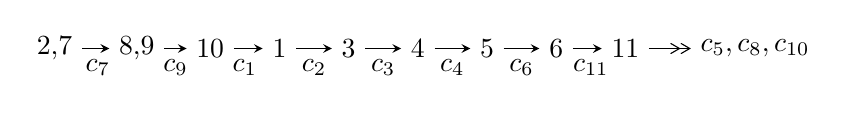
\begin{tikzpicture}[x=25pt, y=7pt]
	% node
	\node (A0) at (-1/8, 0) {2,7};
	\node (A1) at (17/16, 0) {8,9};
	\node (A2) at (17/8, 0) {10};
	\node (A3) at (25/8, 0) {1};
	\node (A4) at (33/8, 0) {3};
	\node (A5) at (41/8, 0) {4};
	\node (A6) at (49/8, 0) {5};
	\node (A7) at (57/8, 0) {6};
	\node (A8) at (65/8, 0) {11};
	\node (C1) at (1/2, -1) {$c_{7}$};
	\node (C2) at (13/8, -1) {$c_{9}$};
	\node (C3) at (21/8, -1) {$c_{1}$};
	\node (C4) at (29/8, -1) {$c_{2}$};
	\node (C5) at (37/8, -1) {$c_{3}$};
	\node (C6) at (45/8, -1) {$c_{4}$};
	\node (C7) at (53/8, -1) {$c_{6}$};
	\node (C8) at (61/8, -1) {$c_{11}$};
	\node (A9) at (10, 0) {$c_{5},c_{8},c_{10}$};

	% edge
	\draw[->,>=stealth]	
	(A0) edge (A1) (A1) edge (A2) (A2) edge (A3) (A3) edge (A4) (A4) edge (A5) (A5) edge (A6) (A6) edge (A7) (A7) edge (A8) ;
	\draw[->>,>={angle 60}]	
	(A8) edge (A9);
\end{tikzpicture} \\ 

\end{tabular} \\

\footnotetext{
The image of knot diagram is generated by the software ``\textbf{Draw programme}" developed by Andrew Bartholomew(\url{http://www.layer8.co.uk/maths/draw/index.htm\#Running-draw}), where we modified some parts for our purpose(\url{https://github.com/CATsTAILs/LinksPainter}).
}\phantom \\ \newline 
\centering \textbf{Ideals for irreducible components\footnotemark of $X_{\text{par}}$} 
 
\begin{align*}
I^u_{1}&=\langle 
- u^{12}+u^{11}- u^{10}+2 u^9-6 u^8+5 u^7- u^6+4 u^5-6 u^4+4 u^3+6 u^2+4 b+1,\\
\phantom{I^u_{1}}&\phantom{= \langle  }- u^{12}+u^{11}- u^{10}+2 u^9-6 u^8+5 u^7- u^6+4 u^5-10 u^4+4 u^3+2 u^2+4 a-3,\\
\phantom{I^u_{1}}&\phantom{= \langle  }u^{13}+2 u^{11}- u^{10}+6 u^9- u^8+6 u^7-3 u^6+8 u^5+4 u^3+u+1\rangle \\
I^u_{2}&=\langle 
2336 u^{15}-694 u^{14}+\cdots+13139 b-13544,\;-7442 u^{15}+7948 u^{14}+\cdots+65695 a+191727,\\
\phantom{I^u_{2}}&\phantom{= \langle  }u^{16}+u^{15}+\cdots+4 u+5\rangle \\
I^u_{3}&=\langle 
b- a-1,\;a^2- a u+2 a- u+2,\;u^2+1\rangle \\
\\
\end{align*}
\raggedright * 3 irreducible components of $\dim_{\mathbb{C}}=0$, with total 33 representations.\\
\footnotetext{All coefficients of polynomials are rational numbers. But the coefficients are sometimes approximated in decimal forms when there is not enough margin.}
\newpage
\renewcommand{\arraystretch}{1}
\centering \section*{I. $I^u_{1}= \langle - u^{12}+u^{11}+\cdots+4 b+1,\;- u^{12}+u^{11}+\cdots+4 a-3,\;u^{13}+2 u^{11}+\cdots+u+1 \rangle$}
\flushleft \textbf{(i) Arc colorings}\\
\begin{tabular}{m{7pt} m{180pt} m{7pt} m{180pt} }
\flushright $a_{2}=$&$\begin{pmatrix}0\\u\end{pmatrix}$ \\
\flushright $a_{7}=$&$\begin{pmatrix}1\\0\end{pmatrix}$ \\
\flushright $a_{8}=$&$\begin{pmatrix}1\\- u^2\end{pmatrix}$ \\
\flushright $a_{9}=$&$\begin{pmatrix}\frac{1}{4} u^{12}-\frac{1}{4} u^{11}+\cdots-\frac{1}{2} u^2+\frac{3}{4}\\\frac{1}{4} u^{12}-\frac{1}{4} u^{11}+\cdots-\frac{3}{2} u^2-\frac{1}{4}\end{pmatrix}$ \\
\flushright $a_{10}=$&$\begin{pmatrix}\frac{1}{2} u^{12}-\frac{1}{2} u^{11}+\cdots-2 u^2+\frac{1}{2}\\\frac{1}{4} u^{12}-\frac{1}{4} u^{11}+\cdots-\frac{3}{2} u^2-\frac{1}{4}\end{pmatrix}$ \\
\flushright $a_{1}=$&$\begin{pmatrix}- u\\u^3+u\end{pmatrix}$ \\
\flushright $a_{3}=$&$\begin{pmatrix}- u^3\\u^5+u^3+u\end{pmatrix}$ \\
\flushright $a_{4}=$&$\begin{pmatrix}-\frac{1}{4} u^{12}-\frac{1}{4} u^{11}+\cdots+\frac{1}{2} u-\frac{1}{4}\\-\frac{1}{4} u^{12}-\frac{1}{4} u^{11}+\cdots+\frac{1}{2} u-\frac{1}{4}\end{pmatrix}$ \\
\flushright $a_{5}=$&$\begin{pmatrix}-\frac{1}{4} u^{12}-\frac{1}{4} u^{11}+\cdots+\frac{3}{2} u-\frac{1}{4}\\-\frac{1}{4} u^{12}-\frac{1}{4} u^{11}+\cdots+\frac{1}{2} u-\frac{1}{4}\end{pmatrix}$ \\
\flushright $a_{6}=$&$\begin{pmatrix}\frac{1}{4} u^{12}-\frac{5}{4} u^{11}+\cdots- u-\frac{5}{4}\\-\frac{1}{2} u^{11}+\frac{1}{2} u^{10}+\cdots-\frac{1}{2} u-1\end{pmatrix}$ \\
\flushright $a_{11}=$&$\begin{pmatrix}-\frac{5}{4} u^{12}-\frac{1}{4} u^{11}+\cdots-\frac{5}{2} u-\frac{3}{4}\\- u^{12}-\frac{3}{2} u^{10}+\cdots- u-\frac{1}{2}\end{pmatrix}$\\ \flushright $a_{11}=$&$\begin{pmatrix}-\frac{5}{4} u^{12}-\frac{1}{4} u^{11}+\cdots-\frac{5}{2} u-\frac{3}{4}\\- u^{12}-\frac{3}{2} u^{10}+\cdots- u-\frac{1}{2}\end{pmatrix}$\\&\end{tabular}
\flushleft \textbf{(ii) Obstruction class $= -1$}\\~\\
\flushleft \textbf{(iii) Cusp Shapes $= 3 u^{12}-3 u^{11}+6 u^{10}-9 u^9+20 u^8-20 u^7+19 u^6-24 u^5+29 u^4-20 u^3+7 u^2-8 u+6$}\\~\\
\newpage\renewcommand{\arraystretch}{1}
\flushleft \textbf{(iv) u-Polynomials at the component}\newline \\
\begin{tabular}{m{50pt}|m{274pt}}
Crossings & \hspace{64pt}u-Polynomials at each crossing \\
\hline $$\begin{aligned}c_{1},c_{3},c_{4}\\c_{7},c_{8}\end{aligned}$$&$\begin{aligned}
&u^{13}+2 u^{11}+u^{10}+6 u^9+u^8+6 u^7+3 u^6+8 u^5+4 u^3+u-1
\end{aligned}$\\
\hline $$\begin{aligned}c_{2}\end{aligned}$$&$\begin{aligned}
&u^{13}+4 u^{12}+\cdots+u-1
\end{aligned}$\\
\hline $$\begin{aligned}c_{5},c_{6},c_{9}\\c_{10}\end{aligned}$$&$\begin{aligned}
&u^{13}+3 u^{12}+\cdots-3 u-2
\end{aligned}$\\
\hline $$\begin{aligned}c_{11}\end{aligned}$$&$\begin{aligned}
&u^{13}-3 u^{12}+\cdots+41 u-24
\end{aligned}$\\
\hline
\end{tabular}\\~\\
\newpage\renewcommand{\arraystretch}{1}
\flushleft \textbf{(v) Riley Polynomials at the component}\newline \\
\begin{tabular}{m{50pt}|m{274pt}}
Crossings & \hspace{64pt}Riley Polynomials at each crossing \\
\hline $$\begin{aligned}c_{1},c_{3},c_{4}\\c_{7},c_{8}\end{aligned}$$&$\begin{aligned}
&y^{13}+4 y^{12}+\cdots+y-1
\end{aligned}$\\
\hline $$\begin{aligned}c_{2}\end{aligned}$$&$\begin{aligned}
&y^{13}+16 y^{12}+\cdots+17 y-1
\end{aligned}$\\
\hline $$\begin{aligned}c_{5},c_{6},c_{9}\\c_{10}\end{aligned}$$&$\begin{aligned}
&y^{13}+15 y^{12}+\cdots+17 y-4
\end{aligned}$\\
\hline $$\begin{aligned}c_{11}\end{aligned}$$&$\begin{aligned}
&y^{13}+3 y^{12}+\cdots+6385 y-576
\end{aligned}$\\
\hline
\end{tabular}\\~\\
\newpage\flushleft \textbf{(vi) Complex Volumes and Cusp Shapes}
$$\begin{array}{c|c|c}  
\text{Solutions to }I^u_{1}& \I (\text{vol} + \sqrt{-1}CS) & \text{Cusp shape}\\
 \hline 
\begin{aligned}
u &= \phantom{-}0.849803 + 0.688633 I \\
a &= \phantom{-}0.100600 + 0.370738 I \\
b &= \phantom{-}0.161020 - 1.380070 I\end{aligned}
 & -2.33364 + 0.79324 I & \phantom{-}4.73185 - 2.01069 I \\ \hline\begin{aligned}
u &= \phantom{-}0.849803 - 0.688633 I \\
a &= \phantom{-}0.100600 - 0.370738 I \\
b &= \phantom{-}0.161020 + 1.380070 I\end{aligned}
 & -2.33364 - 0.79324 I & \phantom{-}4.73185 + 2.01069 I \\ \hline\begin{aligned}
u &= -0.301931 + 0.795374 I \\
a &= \phantom{-}0.53836 + 1.69819 I \\
b &= \phantom{-}0.01733 + 1.65836 I\end{aligned}
 & -11.18850 - 1.28224 I & \phantom{-}2.05046 + 5.61257 I \\ \hline\begin{aligned}
u &= -0.301931 - 0.795374 I \\
a &= \phantom{-}0.53836 - 1.69819 I \\
b &= \phantom{-}0.01733 - 1.65836 I\end{aligned}
 & -11.18850 + 1.28224 I & \phantom{-}2.05046 - 5.61257 I \\ \hline\begin{aligned}
u &= -0.793875 + 0.936102 I \\
a &= -0.703154 - 0.416062 I \\
b &= \phantom{-}0.691430 + 0.338829 I\end{aligned}
 & \phantom{-}3.03190 - 3.86102 I & \phantom{-}7.31704 + 2.47395 I \\ \hline\begin{aligned}
u &= -0.793875 - 0.936102 I \\
a &= -0.703154 + 0.416062 I \\
b &= \phantom{-}0.691430 - 0.338829 I\end{aligned}
 & \phantom{-}3.03190 + 3.86102 I & \phantom{-}7.31704 - 2.47395 I \\ \hline\begin{aligned}
u &= \phantom{-}0.426416 + 0.596732 I \\
a &= \phantom{-}0.581070 - 0.572912 I \\
b &= -0.016047 - 0.904459 I\end{aligned}
 & -2.28202 + 1.46619 I & \phantom{-}3.02331 - 4.77758 I \\ \hline\begin{aligned}
u &= \phantom{-}0.426416 - 0.596732 I \\
a &= \phantom{-}0.581070 + 0.572912 I \\
b &= -0.016047 + 0.904459 I\end{aligned}
 & -2.28202 - 1.46619 I & \phantom{-}3.02331 + 4.77758 I \\ \hline\begin{aligned}
u &= \phantom{-}0.760740 + 1.064260 I \\
a &= -1.237650 + 0.471225 I \\
b &= \phantom{-}0.631392 + 0.645827 I\end{aligned}
 & \phantom{-}2.12458 + 8.30943 I & \phantom{-}4.97203 - 7.67433 I \\ \hline\begin{aligned}
u &= \phantom{-}0.760740 - 1.064260 I \\
a &= -1.237650 - 0.471225 I \\
b &= \phantom{-}0.631392 - 0.645827 I\end{aligned}
 & \phantom{-}2.12458 - 8.30943 I & \phantom{-}4.97203 + 7.67433 I\\
 \hline 
 \end{array}$$\newpage$$\begin{array}{c|c|c}  
\text{Solutions to }I^u_{1}& \I (\text{vol} + \sqrt{-1}CS) & \text{Cusp shape}\\
 \hline 
\begin{aligned}
u &= -0.717554 + 1.160670 I \\
a &= -1.71256 - 0.47703 I \\
b &= \phantom{-}0.20153 - 1.58392 I\end{aligned}
 & -5.31862 - 11.41160 I & \phantom{-}1.59544 + 6.78413 I \\ \hline\begin{aligned}
u &= -0.717554 - 1.160670 I \\
a &= -1.71256 + 0.47703 I \\
b &= \phantom{-}0.20153 + 1.58392 I\end{aligned}
 & -5.31862 + 11.41160 I & \phantom{-}1.59544 - 6.78413 I \\ \hline\begin{aligned}
u &= -0.447199\phantom{ +0.000000I} \\
a &= \phantom{-}0.866672\phantom{ +0.000000I} \\
b &= -0.373309\phantom{ +0.000000I}\end{aligned}
 & \phantom{-}0.678852\phantom{ +0.000000I} & \phantom{-}14.6200\phantom{ +0.000000I}\\
 \hline 
 \end{array}$$\newpage\newpage\renewcommand{\arraystretch}{1}
\centering \section*{II. $I^u_{2}= \langle 2336 u^{15}-694 u^{14}+\cdots+13139 b-13544,\;-7442 u^{15}+7948 u^{14}+\cdots+65695 a+191727,\;u^{16}+u^{15}+\cdots+4 u+5 \rangle$}
\flushleft \textbf{(i) Arc colorings}\\
\begin{tabular}{m{7pt} m{180pt} m{7pt} m{180pt} }
\flushright $a_{2}=$&$\begin{pmatrix}0\\u\end{pmatrix}$ \\
\flushright $a_{7}=$&$\begin{pmatrix}1\\0\end{pmatrix}$ \\
\flushright $a_{8}=$&$\begin{pmatrix}1\\- u^2\end{pmatrix}$ \\
\flushright $a_{9}=$&$\begin{pmatrix}0.113281 u^{15}-0.120983 u^{14}+\cdots-0.144562 u-2.91844\\-0.177791 u^{15}+0.0528198 u^{14}+\cdots-0.306035 u+1.03082\end{pmatrix}$ \\
\flushright $a_{10}=$&$\begin{pmatrix}-0.0645102 u^{15}-0.0681635 u^{14}+\cdots-0.450597 u-1.88762\\-0.177791 u^{15}+0.0528198 u^{14}+\cdots-0.306035 u+1.03082\end{pmatrix}$ \\
\flushright $a_{1}=$&$\begin{pmatrix}- u\\u^3+u\end{pmatrix}$ \\
\flushright $a_{3}=$&$\begin{pmatrix}- u^3\\u^5+u^3+u\end{pmatrix}$ \\
\flushright $a_{4}=$&$\begin{pmatrix}0.440429 u^{15}+0.374290 u^{14}+\cdots+5.23398 u+1.69710\\-0.246594 u^{15}-0.358246 u^{14}+\cdots-0.496385 u-1.22780\end{pmatrix}$ \\
\flushright $a_{5}=$&$\begin{pmatrix}\frac{1}{5} u^{15}+\frac{1}{5} u^{14}+\cdots+\frac{14}{5} u+\frac{4}{5}\\-0.240429 u^{15}-0.174290 u^{14}+\cdots-1.43398 u-0.897100\end{pmatrix}$ \\
\flushright $a_{6}=$&$\begin{pmatrix}0.0488926 u^{15}-0.264525 u^{14}+\cdots-0.240840 u-0.483477\\-0.287236 u^{15}-0.200624 u^{14}+\cdots-0.500419 u-0.889413\end{pmatrix}$ \\
\flushright $a_{11}=$&$\begin{pmatrix}0.206165 u^{15}+0.383956 u^{14}+\cdots+0.862410 u+1.13069\\-0.0159830 u^{15}-0.106553 u^{14}+\cdots+1.24560 u-0.338839\end{pmatrix}$\\ \flushright $a_{11}=$&$\begin{pmatrix}0.206165 u^{15}+0.383956 u^{14}+\cdots+0.862410 u+1.13069\\-0.0159830 u^{15}-0.106553 u^{14}+\cdots+1.24560 u-0.338839\end{pmatrix}$\\&\end{tabular}
\flushleft \textbf{(ii) Obstruction class $= -1$}\\~\\
\flushleft \textbf{(iii) Cusp Shapes $= \frac{488}{1877} u^{15}-\frac{1752}{1877} u^{14}+\cdots-\frac{16008}{1877} u-\frac{9926}{1877}$}\\~\\
\newpage\renewcommand{\arraystretch}{1}
\flushleft \textbf{(iv) u-Polynomials at the component}\newline \\
\begin{tabular}{m{50pt}|m{274pt}}
Crossings & \hspace{64pt}u-Polynomials at each crossing \\
\hline $$\begin{aligned}c_{1},c_{3},c_{4}\\c_{7},c_{8}\end{aligned}$$&$\begin{aligned}
&u^{16}- u^{15}+\cdots-4 u+5
\end{aligned}$\\
\hline $$\begin{aligned}c_{2}\end{aligned}$$&$\begin{aligned}
&u^{16}+7 u^{15}+\cdots+124 u+25
\end{aligned}$\\
\hline $$\begin{aligned}c_{5},c_{6},c_{9}\\c_{10},c_{11}\end{aligned}$$&$\begin{aligned}
&(u^8- u^7+5 u^6-4 u^5+7 u^4-4 u^3+2 u^2+1)^2
\end{aligned}$\\
\hline
\end{tabular}\\~\\
\newpage\renewcommand{\arraystretch}{1}
\flushleft \textbf{(v) Riley Polynomials at the component}\newline \\
\begin{tabular}{m{50pt}|m{274pt}}
Crossings & \hspace{64pt}Riley Polynomials at each crossing \\
\hline $$\begin{aligned}c_{1},c_{3},c_{4}\\c_{7},c_{8}\end{aligned}$$&$\begin{aligned}
&y^{16}+7 y^{15}+\cdots+124 y+25
\end{aligned}$\\
\hline $$\begin{aligned}c_{2}\end{aligned}$$&$\begin{aligned}
&y^{16}+3 y^{15}+\cdots+824 y+625
\end{aligned}$\\
\hline $$\begin{aligned}c_{5},c_{6},c_{9}\\c_{10},c_{11}\end{aligned}$$&$\begin{aligned}
&(y^8+9 y^7+31 y^6+50 y^5+39 y^4+22 y^3+18 y^2+4 y+1)^2
\end{aligned}$\\
\hline
\end{tabular}\\~\\
\newpage\flushleft \textbf{(vi) Complex Volumes and Cusp Shapes}
$$\begin{array}{c|c|c}  
\text{Solutions to }I^u_{2}& \I (\text{vol} + \sqrt{-1}CS) & \text{Cusp shape}\\
 \hline 
\begin{aligned}
u &= -0.548614 + 0.832668 I \\
a &= -1.83759 + 1.08227 I \\
b &= \phantom{-}0.06382 - 1.51723 I\end{aligned}
 & -9.89946 - 2.18536 I & \phantom{-}0.41681 + 3.14055 I \\ \hline\begin{aligned}
u &= -0.548614 - 0.832668 I \\
a &= -1.83759 - 1.08227 I \\
b &= \phantom{-}0.06382 + 1.51723 I\end{aligned}
 & -9.89946 + 2.18536 I & \phantom{-}0.41681 - 3.14055 I \\ \hline\begin{aligned}
u &= -0.969644 + 0.496042 I \\
a &= \phantom{-}0.353364 + 0.413115 I \\
b &= -0.19980 - 1.51366 I\end{aligned}
 & -3.28987 + 5.23868 I & \phantom{-}4.00000 - 3.04258 I \\ \hline\begin{aligned}
u &= -0.969644 - 0.496042 I \\
a &= \phantom{-}0.353364 - 0.413115 I \\
b &= -0.19980 + 1.51366 I\end{aligned}
 & -3.28987 - 5.23868 I & \phantom{-}4.00000 + 3.04258 I \\ \hline\begin{aligned}
u &= \phantom{-}0.886697 + 0.673651 I \\
a &= \phantom{-}0.835367 - 0.338086 I \\
b &= -0.647085 + 0.502738 I\end{aligned}
 & \phantom{-}3.31972 - 2.18536 I & \phantom{-}7.58319 + 3.14055 I \\ \hline\begin{aligned}
u &= \phantom{-}0.886697 - 0.673651 I \\
a &= \phantom{-}0.835367 + 0.338086 I \\
b &= -0.647085 - 0.502738 I\end{aligned}
 & \phantom{-}3.31972 + 2.18536 I & \phantom{-}7.58319 - 3.14055 I \\ \hline\begin{aligned}
u &= -0.822874 + 0.843581 I \\
a &= \phantom{-}1.216240 + 0.256877 I \\
b &= -0.647085 + 0.502738 I\end{aligned}
 & \phantom{-}3.31972 - 2.18536 I & \phantom{-}7.58319 + 3.14055 I \\ \hline\begin{aligned}
u &= -0.822874 - 0.843581 I \\
a &= \phantom{-}1.216240 - 0.256877 I \\
b &= -0.647085 - 0.502738 I\end{aligned}
 & \phantom{-}3.31972 + 2.18536 I & \phantom{-}7.58319 - 3.14055 I \\ \hline\begin{aligned}
u &= \phantom{-}0.043421 + 1.182100 I \\
a &= -0.104055 - 0.579236 I \\
b &= \phantom{-}0.283060 - 0.443755 I\end{aligned}
 & -3.28987 - 1.04600 I & \phantom{-}4.00000 + 6.68545 I \\ \hline\begin{aligned}
u &= \phantom{-}0.043421 - 1.182100 I \\
a &= -0.104055 + 0.579236 I \\
b &= \phantom{-}0.283060 + 0.443755 I\end{aligned}
 & -3.28987 + 1.04600 I & \phantom{-}4.00000 - 6.68545 I\\
 \hline 
 \end{array}$$\newpage$$\begin{array}{c|c|c}  
\text{Solutions to }I^u_{2}& \I (\text{vol} + \sqrt{-1}CS) & \text{Cusp shape}\\
 \hline 
\begin{aligned}
u &= \phantom{-}0.239639 + 0.738346 I \\
a &= -1.82664 - 0.62597 I \\
b &= \phantom{-}0.283060 + 0.443755 I\end{aligned}
 & -3.28987 + 1.04600 I & \phantom{-}4.00000 - 6.68545 I \\ \hline\begin{aligned}
u &= \phantom{-}0.239639 - 0.738346 I \\
a &= -1.82664 + 0.62597 I \\
b &= \phantom{-}0.283060 - 0.443755 I\end{aligned}
 & -3.28987 - 1.04600 I & \phantom{-}4.00000 + 6.68545 I \\ \hline\begin{aligned}
u &= \phantom{-}0.769845 + 1.017620 I \\
a &= \phantom{-}1.54571 - 0.12141 I \\
b &= -0.19980 - 1.51366 I\end{aligned}
 & -3.28987 + 5.23868 I & \phantom{-}4.00000 - 3.04258 I \\ \hline\begin{aligned}
u &= \phantom{-}0.769845 - 1.017620 I \\
a &= \phantom{-}1.54571 + 0.12141 I \\
b &= -0.19980 + 1.51366 I\end{aligned}
 & -3.28987 - 5.23868 I & \phantom{-}4.00000 + 3.04258 I \\ \hline\begin{aligned}
u &= -0.098471 + 1.335410 I \\
a &= \phantom{-}0.017611 + 1.367960 I \\
b &= \phantom{-}0.06382 + 1.51723 I\end{aligned}
 & -9.89946 + 2.18536 I & \phantom{-}0.41681 - 3.14055 I \\ \hline\begin{aligned}
u &= -0.098471 - 1.335410 I \\
a &= \phantom{-}0.017611 - 1.367960 I \\
b &= \phantom{-}0.06382 - 1.51723 I\end{aligned}
 & -9.89946 - 2.18536 I & \phantom{-}0.41681 + 3.14055 I\\
 \hline 
 \end{array}$$\newpage\newpage\renewcommand{\arraystretch}{1}
\centering \section*{III. $I^u_{3}= \langle b- a-1,\;a^2- a u+2 a- u+2,\;u^2+1 \rangle$}
\flushleft \textbf{(i) Arc colorings}\\
\begin{tabular}{m{7pt} m{180pt} m{7pt} m{180pt} }
\flushright $a_{2}=$&$\begin{pmatrix}0\\u\end{pmatrix}$ \\
\flushright $a_{7}=$&$\begin{pmatrix}1\\0\end{pmatrix}$ \\
\flushright $a_{8}=$&$\begin{pmatrix}1\\1\end{pmatrix}$ \\
\flushright $a_{9}=$&$\begin{pmatrix}a\\a+1\end{pmatrix}$ \\
\flushright $a_{10}=$&$\begin{pmatrix}2 a+1\\a+1\end{pmatrix}$ \\
\flushright $a_{1}=$&$\begin{pmatrix}- u\\0\end{pmatrix}$ \\
\flushright $a_{3}=$&$\begin{pmatrix}u\\u\end{pmatrix}$ \\
\flushright $a_{4}=$&$\begin{pmatrix}- a u+u\\- a u\end{pmatrix}$ \\
\flushright $a_{5}=$&$\begin{pmatrix}- a u\\- a u- u\end{pmatrix}$ \\
\flushright $a_{6}=$&$\begin{pmatrix}2 a u- a+2 u-2\\a u+u-1\end{pmatrix}$ \\
\flushright $a_{11}=$&$\begin{pmatrix}- a u- a-3 u-1\\- a- u-1\end{pmatrix}$\\ \flushright $a_{11}=$&$\begin{pmatrix}- a u- a-3 u-1\\- a- u-1\end{pmatrix}$\\&\end{tabular}
\flushleft \textbf{(ii) Obstruction class $= 1$}\\~\\
\flushleft \textbf{(iii) Cusp Shapes $= -4$}\\~\\
\newpage\renewcommand{\arraystretch}{1}
\flushleft \textbf{(iv) u-Polynomials at the component}\newline \\
\begin{tabular}{m{50pt}|m{274pt}}
Crossings & \hspace{64pt}u-Polynomials at each crossing \\
\hline $$\begin{aligned}c_{1},c_{3},c_{4}\\c_{7},c_{8}\end{aligned}$$&$\begin{aligned}
&(u^2+1)^2
\end{aligned}$\\
\hline $$\begin{aligned}c_{2}\end{aligned}$$&$\begin{aligned}
&(u+1)^4
\end{aligned}$\\
\hline $$\begin{aligned}c_{5},c_{6},c_{9}\\c_{10}\end{aligned}$$&$\begin{aligned}
&u^4+3 u^2+1
\end{aligned}$\\
\hline $$\begin{aligned}c_{11}\end{aligned}$$&$\begin{aligned}
&(u^2- u-1)^2
\end{aligned}$\\
\hline
\end{tabular}\\~\\
\newpage\renewcommand{\arraystretch}{1}
\flushleft \textbf{(v) Riley Polynomials at the component}\newline \\
\begin{tabular}{m{50pt}|m{274pt}}
Crossings & \hspace{64pt}Riley Polynomials at each crossing \\
\hline $$\begin{aligned}c_{1},c_{3},c_{4}\\c_{7},c_{8}\end{aligned}$$&$\begin{aligned}
&(y+1)^4
\end{aligned}$\\
\hline $$\begin{aligned}c_{2}\end{aligned}$$&$\begin{aligned}
&(y-1)^4
\end{aligned}$\\
\hline $$\begin{aligned}c_{5},c_{6},c_{9}\\c_{10}\end{aligned}$$&$\begin{aligned}
&(y^2+3 y+1)^2
\end{aligned}$\\
\hline $$\begin{aligned}c_{11}\end{aligned}$$&$\begin{aligned}
&(y^2-3 y+1)^2
\end{aligned}$\\
\hline
\end{tabular}\\~\\
\newpage\flushleft \textbf{(vi) Complex Volumes and Cusp Shapes}
$$\begin{array}{c|c|c}  
\text{Solutions to }I^u_{3}& \I (\text{vol} + \sqrt{-1}CS) & \text{Cusp shape}\\
 \hline 
\begin{aligned}
u &= \phantom{-0.000000 -}1.000000 I \\
a &= -1.000000 - 0.618034 I \\
b &= \phantom{-0.000000 } -0.618034 I\end{aligned}
 & -4.27683\phantom{ +0.000000I} & -4.00000\phantom{ +0.000000I} \\ \hline\begin{aligned}
u &= \phantom{-0.000000 -}1.000000 I \\
a &= -1.00000 + 1.61803 I \\
b &= \phantom{-0.000000 -}1.61803 I\end{aligned}
 & -12.1725\phantom{ +0.000000I} & -4.00000\phantom{ +0.000000I} \\ \hline\begin{aligned}
u &= \phantom{-0.000000 } -1.000000 I \\
a &= -1.000000 + 0.618034 I \\
b &= \phantom{-0.000000 -}0.618034 I\end{aligned}
 & -4.27683\phantom{ +0.000000I} & -4.00000\phantom{ +0.000000I} \\ \hline\begin{aligned}
u &= \phantom{-0.000000 } -1.000000 I \\
a &= -1.00000 - 1.61803 I \\
b &= \phantom{-0.000000 } -1.61803 I\end{aligned}
 & -12.1725\phantom{ +0.000000I} & -4.00000\phantom{ +0.000000I}\\
 \hline 
 \end{array}$$\newpage
\newpage\renewcommand{\arraystretch}{1}
\centering \section*{ IV. u-Polynomials}
\begin{tabular}{m{50pt}|m{274pt}}
Crossings & \hspace{64pt}u-Polynomials at each crossing \\
\hline $$\begin{aligned}c_{1},c_{3},c_{4}\\c_{7},c_{8}\end{aligned}$$&$\begin{aligned}
&(u^2+1)^2(u^{13}+2 u^{11}+u^{10}+6 u^9+u^8+6 u^7+3 u^6+8 u^5+4 u^3+u-1)\\
&\cdot(u^{16}- u^{15}+\cdots-4 u+5)
\end{aligned}$\\
\hline $$\begin{aligned}c_{2}\end{aligned}$$&$\begin{aligned}
&((u+1)^4)(u^{13}+4 u^{12}+\cdots+u-1)(u^{16}+7 u^{15}+\cdots+124 u+25)
\end{aligned}$\\
\hline $$\begin{aligned}c_{5},c_{6},c_{9}\\c_{10}\end{aligned}$$&$\begin{aligned}
&(u^4+3 u^2+1)(u^8- u^7+5 u^6-4 u^5+7 u^4-4 u^3+2 u^2+1)^2\\
&\cdot(u^{13}+3 u^{12}+\cdots-3 u-2)
\end{aligned}$\\
\hline $$\begin{aligned}c_{11}\end{aligned}$$&$\begin{aligned}
&(u^2- u-1)^2(u^8- u^7+5 u^6-4 u^5+7 u^4-4 u^3+2 u^2+1)^2\\
&\cdot(u^{13}-3 u^{12}+\cdots+41 u-24)
\end{aligned}$\\
\hline
\end{tabular}\newpage\renewcommand{\arraystretch}{1}
\centering \section*{ V. Riley Polynomials}
\begin{tabular}{m{50pt}|m{274pt}}
Crossings & \hspace{64pt}Riley Polynomials at each crossing \\
\hline $$\begin{aligned}c_{1},c_{3},c_{4}\\c_{7},c_{8}\end{aligned}$$&$\begin{aligned}
&((y+1)^4)(y^{13}+4 y^{12}+\cdots+y-1)(y^{16}+7 y^{15}+\cdots+124 y+25)
\end{aligned}$\\
\hline $$\begin{aligned}c_{2}\end{aligned}$$&$\begin{aligned}
&((y-1)^4)(y^{13}+16 y^{12}+\cdots+17 y-1)(y^{16}+3 y^{15}+\cdots+824 y+625)
\end{aligned}$\\
\hline $$\begin{aligned}c_{5},c_{6},c_{9}\\c_{10}\end{aligned}$$&$\begin{aligned}
&(y^2+3 y+1)^2\\
&\cdot(y^8+9 y^7+31 y^6+50 y^5+39 y^4+22 y^3+18 y^2+4 y+1)^2\\
&\cdot(y^{13}+15 y^{12}+\cdots+17 y-4)
\end{aligned}$\\
\hline $$\begin{aligned}c_{11}\end{aligned}$$&$\begin{aligned}
&(y^2-3 y+1)^2\\
&\cdot(y^8+9 y^7+31 y^6+50 y^5+39 y^4+22 y^3+18 y^2+4 y+1)^2\\
&\cdot(y^{13}+3 y^{12}+\cdots+6385 y-576)
\end{aligned}$\\
\hline
\end{tabular}
\vskip 2pc
\end{document}